\documentclass[compress, aspectratio=169]{beamer}

%presentation layout

\mode<presentation>
{
  \usetheme{Berlin}
  % \usecolortheme{dove}
  \setbeamercolor{structure}{bg=white,fg=black}
  \setbeamercolor{normal text}{bg=white,fg=black}
  \setbeamercolor{titlepage}{bg=white,fg=black}
  \setbeamercolor{titlelike}{bg=white,fg=black}
  \setbeamercolor{palette primary}{bg=white}
  \setbeamercolor{palette secondary}{bg=gray, fg=white}
  \setbeamercolor{palette tertiary}{bg=gray, fg=white}
  \setbeamercolor{palette quarternary}{bg=white}
  \setbeamercovered{transparent}
  \useinnertheme{rectangles}
  %\usefonttheme{serif}
}

\setbeamertemplate{navigation symbols}{}

%loading packages
\usepackage[ngerman]{babel}
\usepackage[T1]{fontenc}
\usepackage[utf8]{inputenc}
\usepackage{graphicx}
\usepackage{amsmath}
\usepackage{framed}
\usepackage{caption}
\usepackage{subcaption}
\usepackage{multicol} 
\usepackage{xcolor}

\definecolor{light-gray}{gray}{0.97}

% vorgeplaenkel
\title[Endplenum]{Endplenum}

\author{Ständiger Ausschuss aller Physikfachschaften}

\institute[Zusammenkunft aller Physikfachschaften]

\date{15. November 2020}

\subject{Endplenum der OZaPFhiG}

\begin{document}

\section{Begrüßung}

{
\setbeamercolor{background canvas}{bg=light-gray}
\begin{frame}
\begin{figure}
    \centering
    \includegraphics[height=5.5cm]{logo.png}
\end{figure}
\centering
\textbf{Früh aufstehen heißt früh fröhlich sein :)\\ Guten Morgen und willkommen zum Endplenum!}
\end{frame}
}

\begin{frame}{How to Plenum}
Diese ZaPF ist eine ZaPF! Und das ist nicht mal tautologisch.\\
$\Rightarrow$ Die Geschäftsordnung für Plenen der ZaPF findet wieder Anwendung.

\vspace{.5cm}
Meldungen über den Chat:
\begin{itemize}
\item$\quad$\textbf{!}$\quad$ \ \ Meldung
\item$\quad$\textbf{?}$\quad$ \ Verständnisfrage
\item$\quad$\textbf{!!!}$\quad$ Geschäftsordnungs-Antrag
\end{itemize}
\vspace{.5cm}
Nennt zu Beginn eines Redebeitrags bitte Name und Uni.
\end{frame}

\section{Formalia}

\begin{frame}\frametitle{Bestimmung der Redeleitung}

  \begin{figure}
     \begin{subfigure}[t]{0.21\textwidth}
       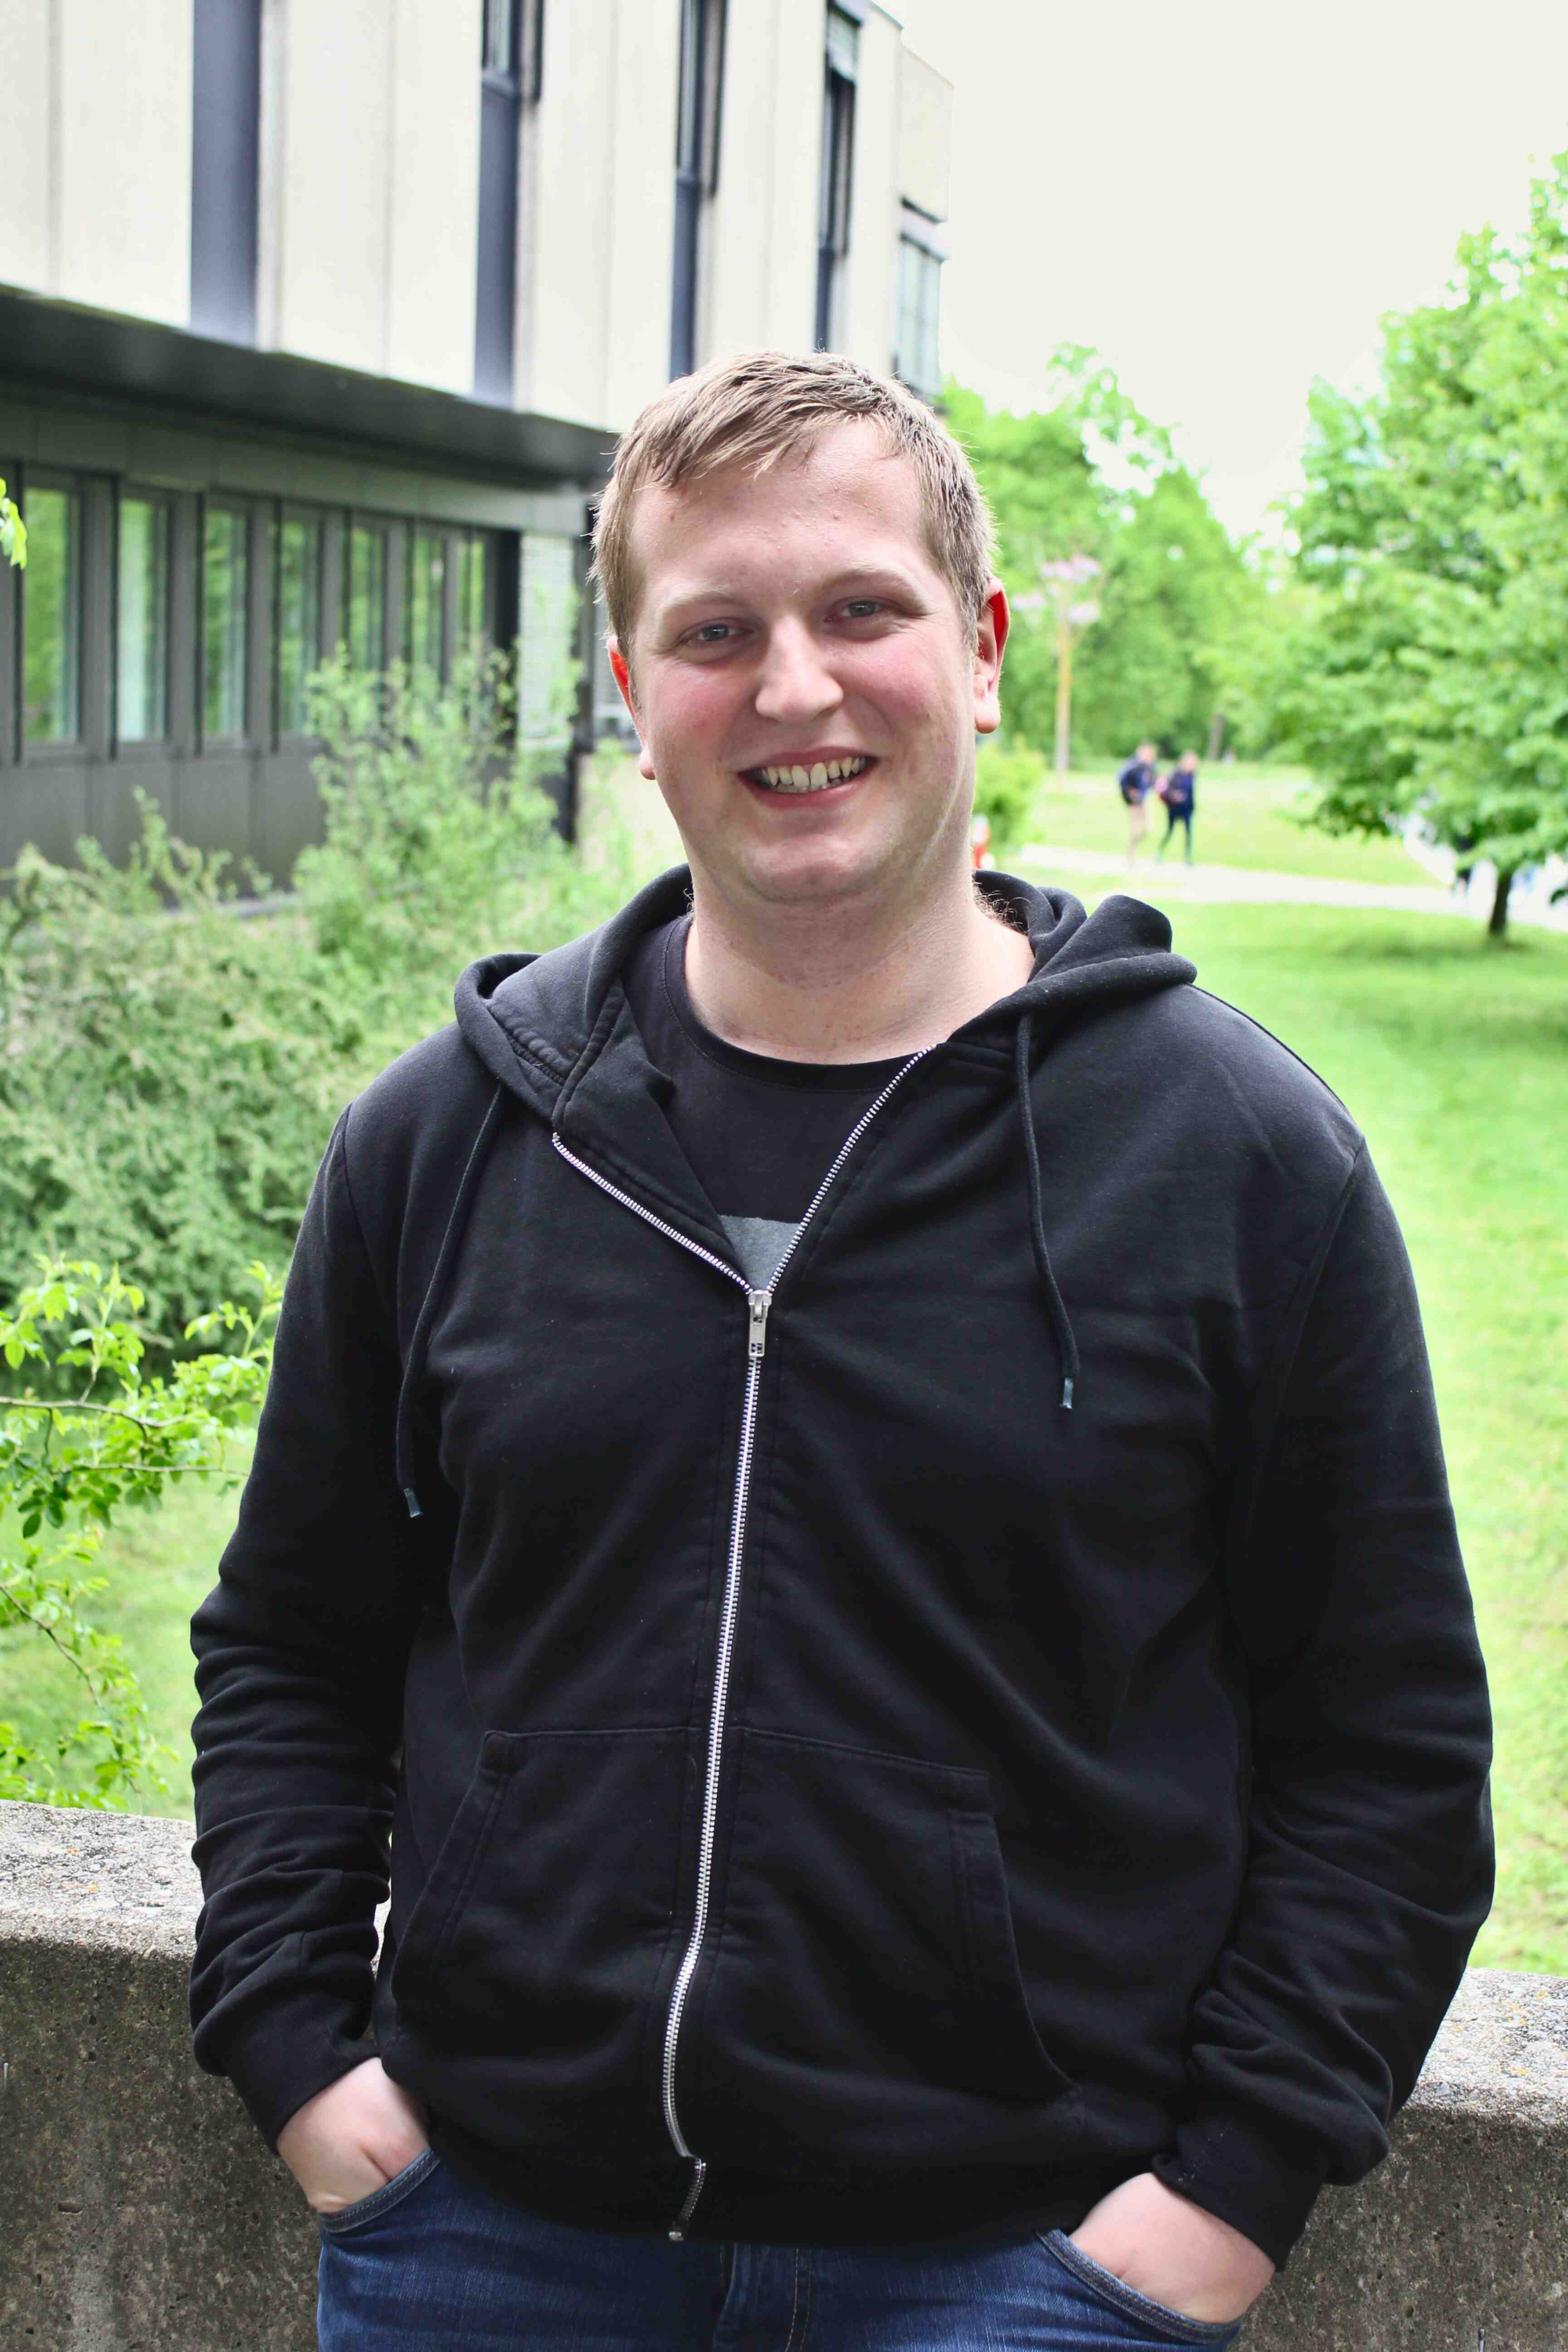
\includegraphics[height=.5\textheight]{max.jpg}
       \caption*{Maximilian Schneider (Würzburg)}
     \end{subfigure}
       \begin{subfigure}[t]{0.3\textwidth}
         
\includegraphics[height=.5\textheight]{leon.jpg}
         \caption*{Leon Nutzinger (FU Berlin)}
     \end{subfigure}
         \begin{subfigure}[t]{0.24\textwidth}
         
\includegraphics[height=.5\textheight]{sean.jpg}
         \caption*{Sean Bonkowski (Bonn)}
     \end{subfigure}
  \end{figure}
 \end{frame}

\begin{frame}{Bestimmung der Protokollführung}
Vorgeschlagene Protokollführung:

\begin{itemize}
\item Christoph Blattgerste (Uni Heidelberg)
\item Victoria Schemenz (Alumna)
\item Niklas Jamborek (Uni Hamburg)
\item Christian Hoffmann (Alumnus)
\item Peter Blum (Uni Hamburg)
\item Niklas Westermann (Uni Konstanz)
\end{itemize}
\end{frame}

\begin{frame}{Feststellung der Beschlussfähigkeit}
Geschäftsordnung (§4): \textit{Die Beschlussfähigkeit für Abstimmungen und Personenwahlen ist gegeben, wenn zwanzig Physikfachschaften im Plenum anwesend sind.}\vspace{.5cm}

Verfahrensvorschlag der Orga: Nutzung eines Abstimmungstools, bei dem der Zugang über das Fachschaftstoken geregelt wird.\vspace{.5cm}

Feststellung der Beschlussfähigkeit: Bitte meldet euch jetzt im Abstimmungstool an und bestätigt eure Anwesenheit.
\end{frame}

\begin{frame}[plain]
\begin{multicols}{2}
    \begin{enumerate}\footnotesize
        \item Begrüßung
	\item Formalia
	\begin{enumerate}
            \item \footnotesize Bestimmung der Redeleitung
            \item Bestimmung der Protokollführung
            \item Feststellung der Beschlussfähigkeit
            \item Beschluss der Tagesordnung
        \end{enumerate}

	\item Wahlen
	\begin{enumerate}
            \item \footnotesize StAPF
            \item TOPF
            \item KomGrem
	    \item Entsendungen in den studentischen Akkreditierungspool
        \end{enumerate}
	\item Vergabe der Sommer-ZaPF 2022
        \item Anträge
	\begin{enumerate}
            \item \footnotesize Resolution zum Entwurf des Bayerischen Hochschulgesetzes
            \item Offener Brief: Präsent bleiben
            \item Resolution zur Einbindung von FDM-Inhalten in der Lehre
            \item Resolution zum barrierefreiem Studium
            \item Resolution zur Überarbeitung der MRVO
            \item Resolution: Umdenken in den Universitäten hin zur Open-Source-Lösungen
            \item Unterstützung Opensourcelms
            \item Datenschutz an die Datenschutzbeauftragten
            \item Datenschutz an die Hochschulen
            \item Datenschutz an die Fachschaften
            \item Mobilitätspositionspapier
            \item Unterstützung des Bündnis 50 Jahre BAföG
        
        \end{enumerate}
	\item Berichte der Arbeitskreise
	\item Kommende ZaPFen
    \item Sonstiges
	\item Auszählung und Veröffentlichung der Wahlergebnisse
    \end{enumerate}
\end{multicols}
\end{frame}


\section{Wahlen}

\begin{frame}{Infos zu Abstimmungen und Wahlen}
\textbf{Offene Abstimmungen}
\begin{itemize}
\item werden über den BBB Chat durchgeführt
\item Personen, die für ihre FS abstimmen sind durch den Namen hervorgehoben
\item Bitte nichts anderes in den Chat schreiben währenddessen!
\end{itemize}
\textbf{Personalwahlen und ggf. geheime Abstimmungen}
\begin{itemize}
\item werden per Briefwahl durchgeführt
\item Die Orga schickt im Anschluss an das Plenum die Wahlunterlagen zu.
\item Die Wahlunterlagen müssen spätestens am 12.06.2021 bei der Orga eingegangen sein.
\item Solange wird das Plenum formell unterbrochen (vor TOP 9) und dann zur Auszählung wieder aufgenommen
\item Auszählung in einem Livestream: 13.06.2021 um 16:00
\end{itemize}
\end{frame}

\begin{frame}{Bestimmung des Wahlausschusses}
Vorschlag:
\begin{itemize}
\item xx
\end{itemize}

\vspace{.5cm}
Ein tosender digitaler Applaus als Akklamation für den Wahlausschuss, der sich auch um die Durchführung der Briefwahl kümmert!
\end{frame}

\begin{frame}{Wahlen}
Zu besetzen sind:\vspace{.5cm}

\textbf{3 Plätze im StAPF}\vspace{.5cm}

\textbf{1 Platz im TOPF}\vspace{.5cm}

\textbf{1 Platz im KomGrem}\vspace{.5cm}

Außerdem wird über Entsendungen in den stud. Akkreditierungspool abgestimmt.
\end{frame}

\section{ZaPF Vergabe Sommer 2022}

\begin{frame}{Vergabe der Sommer-ZaPF 2022}
\centering
%\includegraphics[height=4.5cm]{c10800102ec1324b2188cd572029c8d0.png}

\vspace{.5cm}
\huge Kwak! Wo solls hingehen?
\end{frame}

\section{Anträge}

\begin{frame}
\centering
\huge Resolution zum Entwurf des Bayerischen Hochschulgesetzes
\end{frame}

\begin{frame}
\centering
\huge Offener Brief: Präsent bleiben
\end{frame}

\begin{frame}
\centering
\huge Einbindung von FDM-Inhalten in der Lehre
\end{frame}

\begin{frame}
\centering
\huge Barrierefreies Studium
\end{frame}

\begin{frame}
\centering
\huge Überarbeitung der MRVO
\end{frame}

\begin{frame}
\centering
\huge Umdenken in den Universitäten hin zu Open-Source-Lösungen
\end{frame}

\begin{frame}
\centering
\huge Unterstützung Opensourcelms
\end{frame}

\begin{frame}
\centering
\Large Datenschutzrechtliche Bewertung der Zulässigkeit von //nichteuropäischen// Videokonferenzdiensten und cloudbasierten Diensten im universitären Lehrbetrieb an Datenschutzbeauftragte
\end{frame}

\begin{frame}
\centering
\Large Datenschutzrechtliche Bewertung der Zulässigkeit von //nichteuropäischen// Videokonferenzdiensten und cloudbasierten Diensten im universitären Lehrbetrieb an Hochschulen
\end{frame}

\begin{frame}
\centering
\Large Aufruf an den StaPF den Aufruf an Studierende, lokale Datenschutzbeauftragte zur Prüfung der Datenschutzkonformität von //nichteuropäischen// Videokonferenzdiensten und cloudbasierten Diensten im universitären Lehrbetrieb an Fachschaften im deutschsprachigen Raum weiter zu leiten.
\end{frame}

\begin{frame}
\centering
\huge Mobilitätspositionspapier
\end{frame}


\begin{frame}
\centering
\huge Unterstützung des Bündnis 50 Jahre BAföG - kein Grund zu feiern
\end{frame}


\begin{frame}
\centering
\huge Weitere Anträge?
\end{frame}



\section{Berichte der Arbeitskreise}

\begin{frame}{Vorstellung der Arbeitskreise}
	\begin{itemize}
		\item Bitte fasst euch kurz! (ca. 3 Minuten)
		\item Im Anschluss an die Vorstellung des AKs könnt ihr Fragen stellen.
	\end{itemize}
\end{frame}

\begin{frame}{Arbeitskreise I}
	\begin{itemize}
		\item Mitgliederversammlung ZaPF e.V.
		\item AK Wissenschaftsrecht - Opa, Gabriel (Chemnitz)
		\item AK Klafki für die Hochschule - Amr (HU Berlin), Stefan (Köln)
		\item AK Orga-Austausch - Andy (Würzburg)
	\end{itemize}
\end{frame}

\begin{frame}{Arbeitskreise II}
	\begin{itemize}
		\item Selbstberichtsbewertung - Tobi (Düsseldorf)
		\item Open Source ab Universitäten - Tobi (Düsseldorf)
		\item Open Source Bildungsplattformen - Tobi (Düsseldorf)
		\item Datenschutz Videokonfernzsysteme - Tobi (Düsseldorf)
		\item Wiki Pflege - Tobi (Düsseldorf)
	\end{itemize}
\end{frame}

\begin{frame}{Arbeitskreise III}
	\begin{itemize}
		\item AK Einführung zu Mobilität und Durchlässigkeit - Fabs
		\item AK Gemeinsames PosPa zu Mobilität und Durchlässigkeit -  Fabs
		\item AK Fachschafts-Veranstaltungen - Andy (Würzburg)
		\item AK BaMa-Umfrage - Felicia (Göttingen)
		\item MeTaFa - Vicky (Alumni)
	\end{itemize}
\end{frame}

\begin{frame}{Arbeitskreise IV}
	\begin{itemize}
		\item AK Studiengang-Diagramm Erstellung - Stefan (Köln), Daniela (ehemals Frankfurt)
		\item AK NFDI - Philipp (Alumni)
		\item AK Wissenschaftliche Kariere - Philipp (Alumni)
		\item AK Wissenschaft und Gesellschaft - Philipp (Alumni)
		\item AK Mental Health Umfrage - Philipp (Alumni)
	\end{itemize}
\end{frame}

\begin{frame}{Arbeitskreise V}
	\begin{itemize}
		\item AK Nachhaltigkeit - Daniel (TUM), Katrin (TUM)	
		\item AK Lehramtsumfrage KFP - Sebbo (Heidelberg)
		\item AK Fachschaften und jDPG - Janice (Münster)
		\item Der StAPF stellt sich vor - StAPF
		\item AK Fachschaftsnachwuchs - Laura (Würzburg), Tim (Würzburg) 
	\end{itemize}
\end{frame}

\begin{frame}{Arbeitskreise VI}
	\begin{itemize}
		\item Angemessene Prüfungsformate \& Programmieren - Manu (Wien) 
		\item Hybrid Lehre - Manu (Wien), Amr (HU Berlin)
		\item AK Bayerische Hochschulgesetznovelle - Andy (Würzburg) 
		\item AK Fachschafts-Freundschaften - Andy (Würzburg), Tobi (Düsseldorf)
		\item AK Handreichung zu Mental Health - Anna (Kiel) 
	\end{itemize}
\end{frame}

\begin{frame}{Arbeitskreise VII}
	\begin{itemize}
		\item AK Studienführer 2.0 - Vicky (Alumni) 
		\item AK KommGrem - KommGrem 
		\item AK Lost Generation - tbd
		\item AK Ad Personam Professur und Anforderungen an Professuren - Paul (Köln)
		\item AK Austausch Lehramt - Leon (FU Berlin)
	\end{itemize}
\end{frame}

\begin{frame}{Arbeitskreise VIII}
	\begin{itemize}
		\item AK Evaluation der Lehre - Jules (Hamburg), Markus (Hamburg)
		\item Forschungsorientierte Lehre - Amr (HU Berlin)
		\item Atomwaffen, das Recht des Stärkeren und was wir dagegen in der Hand haben - Christos (ehemals Köln)
		\item AK BAföG - Peter (Alumni)
		\item AK Evaluation MRVO - Philipp (Alumni)
	\end{itemize}
\end{frame}

\section{Kommende ZaPFen}

\begin{frame}{Kommende ZaPFen}
    \begin{figure}
        \centering
      %  \includegraphics[height=4cm]{LOGO-quadratisch-transparent_TIF_2021.png}
        \includegraphics[height=3.2cm]{logo_goettingen.png}
    \end{figure}
    \vspace{0.25cm}
    \centering
    \large Viel Erfolg und vielen Dank an alle ausrichtenden Fachschaften!
\end{frame}

\section{Sonstiges}

\begin{frame}{Sonstiges}
\centering
\huge Habt ihr noch etwas?

\end{frame}

\end{document}
